% !TEX root = ../paper.tex

\section{Introduction}

Infrared-visible alignment is becoming a foundational capability for UAV inspection, monitoring,
and nighttime multimodal perception. Visible imagery provides semantic and structural detail,
while infrared thermal imagery remains informative under illumination changes, smoke, haze, and
low-light conditions. This complementarity has driven progress across multispectral pedestrian
perception, thermal object detection, visible-thermal tracking, and UAV multimodal sensing
\cite{hwang2015kaist,flir2018thermal,jia2021llvip,liu2022tardal,sun2022dronevehicle,zhang2022vtuav,li2022lasher,jiang2023antiuav}.
For these systems to operate as fused sensors rather than separate streams, however, RGB and
thermal observations must be aligned reliably at the scene level.

Real UAV infrared-visible alignment is substantially more demanding than standard same-view image
matching. Aerial platforms introduce viewpoint drift, cross-FOV capture, rolling scale changes, and
cross-resolution sensors; thermal images further introduce low-texture regions, grayscale or
pseudocolor rendering, and strong day/night appearance shifts. These factors make individual
frame-level homographies uneven: some pairs are strongly supported, while others require additional
scene context before they should influence the final transform. The practical question is therefore
not only whether a matcher can produce correspondences for one pair, but whether a system can
decide which scene-level alignment should be trusted.

Recent pairwise matching has advanced rapidly. Transformer, dense, and multimodal matchers such as
LoFTR, LightGlue, DKM, RoMa, XoFTR, and MINIMA have substantially improved correspondence
availability under difficult appearance changes
\cite{sarlin2020superglue,sun2021loftr,chen2022aspanformer,lindenberger2023lightglue,edstedt2023dkm,edstedt2024roma,tuzcuoglu2024xoftr,ren2025minima}.
At the benchmark level, recent UAV visible-infrared alignment studies have also shown that
synthetic transform supervision can support trainable alignment baselines with controlled
geometric metrics \cite{gao2025uavmatch}. UAV-TAlign-12K targets the complementary operating
regime: real captured cross-FOV UAV infrared-visible scenes where the central product is a
retained scene-level transform rather than only a supervised pairwise transform prediction.
Our 12K-scale experiments confirm this progress in the UAV infrared-visible setting: strong
off-the-shelf classical and modern baselines already provide broadly available pairwise homography
evidence on UAV-TAlign-12K. This result creates a concrete
tension: a method can approach saturated pairwise usability while producing only selective
scene-level retention under a strict acceptance rule. Pairwise usability and scene-level
canonical acceptance therefore measure different operating questions and should not be read as the
same success criterion. The key step is to aggregate evidence across a scene, suppress unstable
homographies, and verify whether the final transform should be retained.

Figure~\ref{fig:scene_reliability_principle} illustrates this distinction. Pairwise homographies
can be available for most frames while their support and scene consistency remain uneven; robust
consensus and QA therefore determine whether the resulting scene transform is retained, whereas
the reliability score is used only to rank scenes for operating-profile analysis.

\begin{figure}[t]
\centering
\makebox[\textwidth][c]{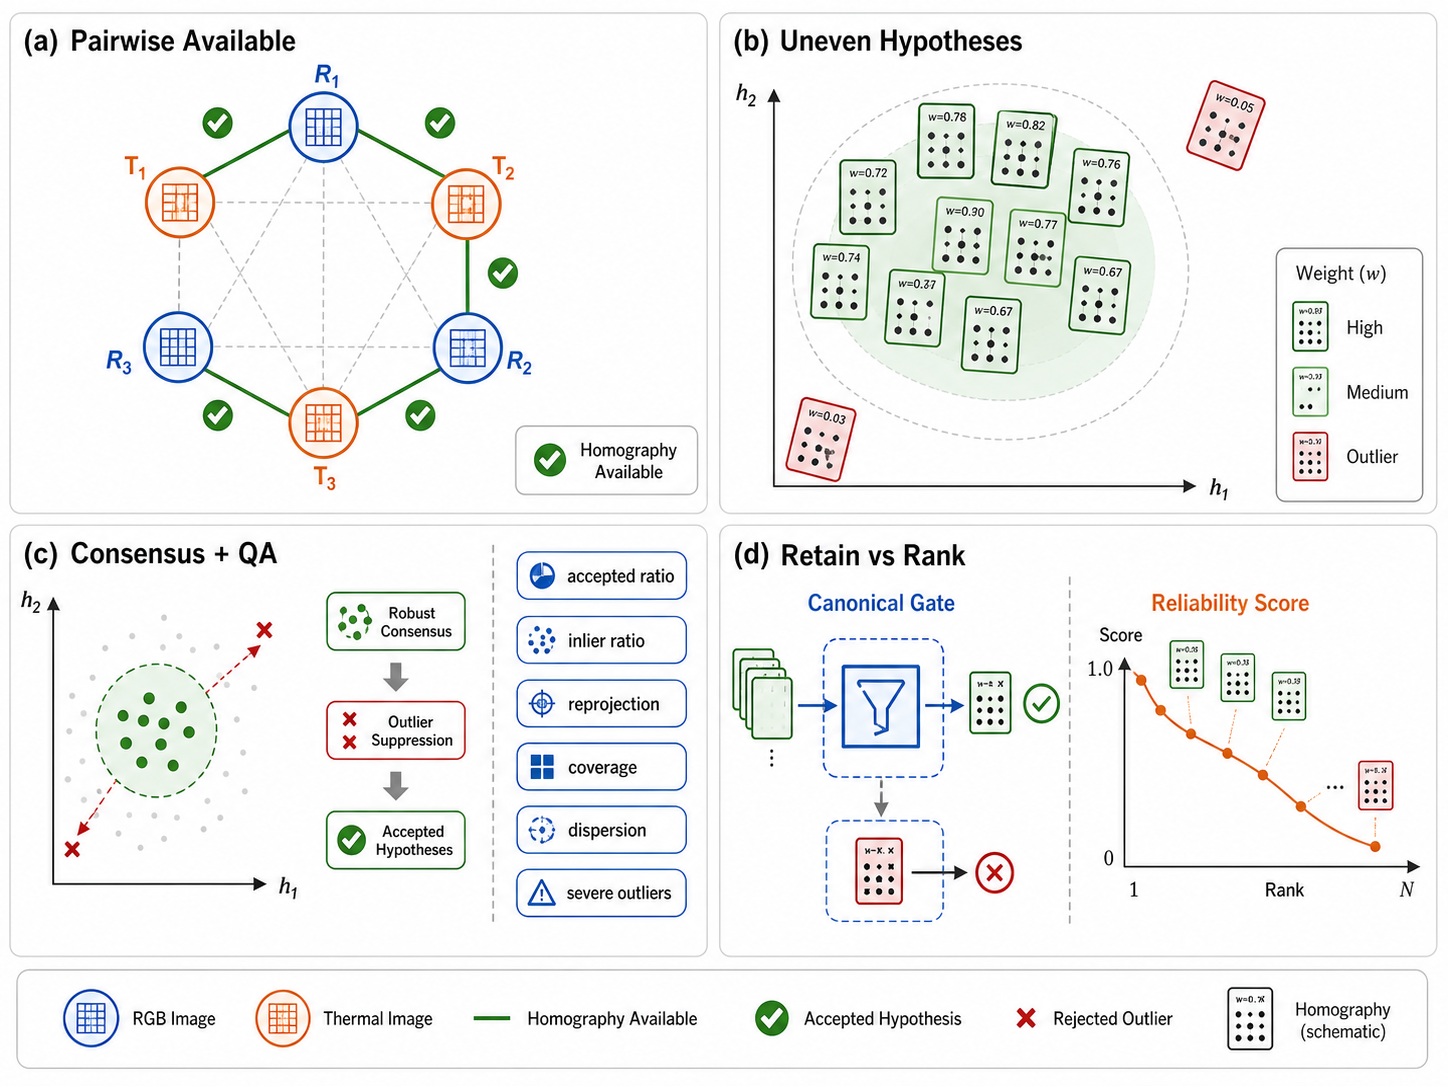
\includegraphics[width=1.05\textwidth]{figures/fig_scene_reliability_principle_image2.png}}
\caption{Principle of scene-level reliability control. Broad pairwise homography availability
does not imply that all frame-level hypotheses are equally trustworthy. UAV-TAlign suppresses
unstable hypotheses, forms a robust scene consensus, and separates the canonical retain/reject
decision from reliability-based ranking.}
\label{fig:scene_reliability_principle}
\end{figure}

This observation motivates a benchmark-first framing with two complementary evaluation questions:
whether a method can produce usable pairwise homography evidence, and whether multi-frame evidence
supports a scene transform that should be retained. Treating these as separate units prevents high
pairwise availability from being interpreted as automatic scene-level reliability.

Our primary contribution is UAV-TAlign-12K, a real-world UAV infrared-visible alignment dataset
with 6,039 candidate pairs and an integrity-checked 6,037-pair evaluation split across 15 scenes.
The collection spans day, night, low-light, grayscale thermal, pseudocolor thermal, and wide,
zoom, and standard UAV views. Its manifest-fixed, label-free protocol evaluates pairwise
homography evidence, canonical scene retention, condition-aware reliability, and risk--coverage
operating profiles. Together, the data and protocol make scene-level alignment reliability
directly studyable under captured cross-FOV UAV conditions.

To instantiate the scene-level benchmark track, we additionally present UAV-TAlign as a reference
alignment method. It operates on top of strong pairwise matchers and uses reliability-guided
evidence selection, robust scene consensus, and QA-aware verification to decide whether a
scene-level transform should be retained. The method contribution is therefore complementary to
the dataset: it provides a reproducible reference implementation for the reliability question
exposed by UAV-TAlign-12K.

Figure~\ref{fig:paper_overview} summarizes the complete paper-level view: UAV-TAlign-12K anchors
pairwise evidence evaluation, UAV-TAlign converts the resulting multi-frame evidence into a
reliability-controlled scene transform, and the protocol reports both canonical retention and the
risk--coverage operating profile.

\begin{figure}[t]
\centering
\makebox[\textwidth][c]{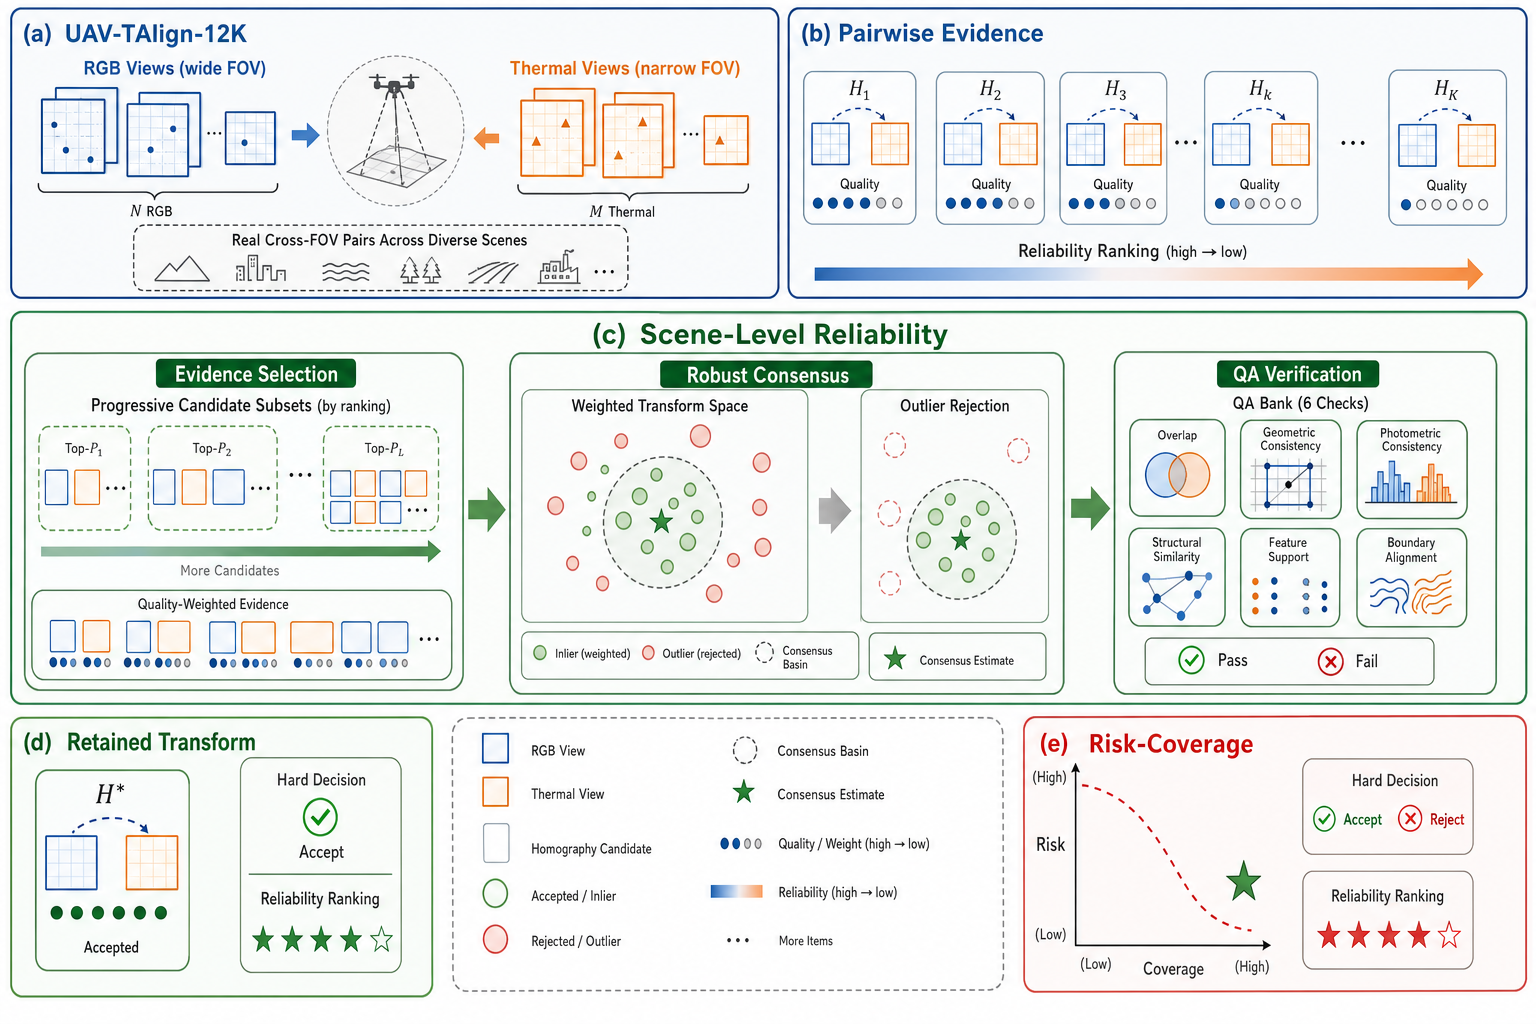
\includegraphics[width=1.15\textwidth]{figures/fig_uav_talign_overview_image2.png}}
\caption{Paper-level overview of UAV-TAlign-12K and UAV-TAlign. The benchmark first measures
pairwise homography evidence, while the reference framework performs scene-level evidence
selection, robust consensus, and QA-aware verification before producing retained alignment
products and reliability--coverage diagnostics.}
\label{fig:paper_overview}
\end{figure}

Our contributions are threefold:
\begin{itemize}
\item We introduce UAV-TAlign-12K, a 6,039-pair real captured cross-FOV UAV infrared-visible
dataset with an integrity-checked 6,037-pair official split across 15 diverse scenes.
\item We establish a manifest-fixed benchmark that separates pairwise homography evidence from
canonical scene-level retention and supports condition-aware and risk--coverage analysis.
\item We provide UAV-TAlign as a scene-level reference method and use classical and modern
off-the-shelf baselines, cumulative ablations, and seed analysis to demonstrate the benchmark's
reliability-centered evaluation capability.
\end{itemize}
